\documentclass[a4,11pt]{aleph-notas}
% Actualizado en febrero de 2024
% Funciona con TeXLive 2022
% Para obtener solo el pdf, compilar con pdfLaTeX. 
% Para obtener el xml compilar con XeLaTeX.

% -- Paquetes adicionales
\usepackage{aleph-comandos}
\usepackage{listings}
\usepackage{xcolor}
\usepackage{mdframed}
\usepackage{verbatim}
\usepackage{textcomp}
\usepackage{mathcomp}
\usepackage{booktabs}
\usepackage{tabularx}

\definecolor{codegreen}{rgb}{0,0.6,0}
\definecolor{codegray}{rgb}{0.5,0.5,0.5}
\definecolor{codepurple}{rgb}{0.58,0,0.82}
\definecolor{backcolour}{rgb}{0.95,0.95,0.92}

\lstdefinestyle{mystyle}{
    backgroundcolor=\color{backcolour},   
    commentstyle=\color{codegreen},
    keywordstyle=\color{magenta},
    numberstyle=\tiny\color{codegray},
    stringstyle=\color{codepurple},
    basicstyle=\ttfamily\footnotesize,
    breakatwhitespace=false,         
    breaklines=true,                 
    captionpos=b,                    
    keepspaces=true,                 
    numbers=left,                    
    numbersep=5pt,                  
    showspaces=false,                
    showstringspaces=false,
    showtabs=false,                  
    tabsize=2
}

% Définition de la commande \ans
% Removed duplicate definition of \ans

% Définition de la commande \ans
\newcommand{\ans}[1]{
\begin{mdframed}[
    roundcorner=10pt,     % Bordures arrondies
    backgroundcolor=gray!20, % Fond gris avec 20% d'opacité
    linecolor=black,      % Couleur de la bordure
    linewidth=1pt,        % Épaisseur de la bordure
    innertopmargin=10pt,  % Marge interne en haut
    innerbottommargin=10pt, % Marge interne en bas
    innerleftmargin=10pt,  % Marge interne à gauche
    innerrightmargin=10pt  % Marge interne à droite
]
#1
\end{mdframed}
}


\lstset{style=mystyle}
% -- Datos 
\institucion{CIRED}
% \carrera{}
\asignatura{Master EEET, parcours modélisation prospective}
\tema{TP8 « scénarios, résultats »}
\autor{Thomas O. Da Costa \& Rachel Pierre-Léandre}
\fecha{\\23 octobre 2024}
\logouno[4.5cm]{Logos/logo_cired}
\definecolor{colortext}{HTML}{05646d}
\definecolor{colordef}{HTML}{00A1DE}
\fuente{montserrat}
% \fuente{mathpazo}

% -- Otros comandos

% Mettre "tema" sur les pages paires et les auterus sur les pages impaires

\begin{document}

\encabezado

\section*{\LARGE{Énoncé}}
\ans{
Vous allez analyser des résultats de scénarios issus du modèle Imaclim-R monde. 

Le document « \textit{ensemble scenarios ImaclimR.pdf} » décrit comment un ensemble de scénarios de « baseline », \textit{i.e.} sans politique climatique, a été obtenu. La base de données de scénarios est enrichie de scénarios « d’atténuation », \textit{i.e.} avec un objectif de réduction des émissions de gaz à effet de serre ; un scénario d’atténuation par baseline. \\

Les résultats correspondants à l’ensemble de ces scénarios en termes d’émissions de CO2 (\textit{ECO2\_w.csv}), de PIB (\textit{GDP\_w.csv}) et de PIB par habitant (\textit{GDPcap\_w.csv}), d’intensité énergétique du PIB (\textit{EI\_w.csv}) et d’intensité carbone de l’énergie (CI\_w.csv), à l’échelle mondiale sur la période 2015-2065, sont fournis dans le dossier \texttt{/data}. Ce dossier contient également les trajectoires de population mondiale, exogène, de l’ensemble des scénarios (\textit{Pop\_w.csv}). Tous les résultats sont donnés en indice par rapport à la valeur 2015. La première ligne donne les années dans les fichiers de résultats. Chaque ligne suivante correspond à un scenario de la base de données de scénarios. Par ailleurs, le dossier contient également un fichier \textit{drivers.csv} qui donne la combinaison des groupes de paramètres correspondant à chaque scénario (voir le fichier \textit{readme.txt} pour une explication des indices du fichier \textit{drivers.csv}). Dans tous les fichiers csv les scénarios sont classés dans le même ordre.  \\

Commencez par lire les différents documents, et par ouvrir les fichiers csv pour comprendre comment les données sont organisées. \\

Vous allez créer et utiliser un code python3 pour lire les données de résultats, et les analyser en traçant un certain nombre de graphiques. Le rendu du TP sera à la fois le code lui-même, et ce fichier dans lequel vous aurez copié vos graphiques et rédigé vos analyses. Merci de mettre des commentaires clairs dans votre code (avec des \# en début de ligne) afin que celui-ci soit lisible.}

\newpage
%%%%%%%%%%%%%%%%%%%%%%%%%%%%%%%%%%%%%%%%
\section*{\LARGE{Compte-rendu}}
%%%%%%%%%%%%%%%%%%%%%%%%%%%%%%%%%%%%%%%%
\section{\Large{{Présentation du modèle Imaclim-R et méthodologie de construction des scénarios}}}
\vspace{0.3cm}

Imaclim-R est un modèle multi-régional et multi-sectoriel de l’économie, conçu pour simuler les trajectoires économiques et énergétiques à l’échelle mondiale. Sa structure hybride et dynamique combine un cadre d’équilibre général calculable (CGE) avec des modules sectoriels, permettant de capturer les interactions complexes entre la macroéconomie, l’énergie et les dynamiques sectorielles (des transports, de l'industrie, etc.). Le modèle prend en compte des imperfections de marché, une utilisation partielle des facteurs de production et des anticipations imparfaites, le distinguant de modèles plus simplifiés. 

Les données utilisées sont calibrées sur l’année de base 2001, ajustées avec les bilans énergétiques de l'Agence Internationale de l'Énergie (AIE) et des informations sur la mobilité des passagers. Le modèle fonctionne sur une structure récursive, avec des équilibres économiques statiques annuels interconnectés, permettant de simuler l’évolution des variables économiques et énergétiques d'année en année.

\subsection{Méthodologie de construction des scénarios}

La construction des scénarios avec Imaclim-R repose sur l’identification de paramètres aux valeurs incertaines influençant simultanément les émissions de GES et la croissance du PIB. Ces paramètres, regroupés en sept catégories, incluent des hypothèses sur la croissance de la productivité, les comportements de la demande énergétique, l’efficacité énergétique, la disponibilité des technologies bas carbone et l’accès aux énergies fossiles non conventionnelles. Pour chaque catégorie, plusieurs valeurs alternatives sont définies, offrant ainsi une large palette de trajectoires économiques et environnementales possibles.

Les scénarios sont donc le résultat de combinaisons d'hypothèses variées, telles que des taux de croissance de productivité différents dans diverses régions ou des comportements contrastés en matière de consommation d’énergie. Le modèle inclut également des dynamiques endogènes liées à l'évolution technologique et au changement structurel, influencées par les prix relatifs et l'apprentissage des technologies émergentes.

\subsection{Principaux choix méthodologiques et leurs limites}

\begin{enumerate}
    \item \textbf{Choix des paramètres et valeurs alternatives} : La construction des scénarios repose sur la sélection de paramètres aux valeurs inconnues (par exemple, la croissance de la productivité, la disponibilité des énergies fossiles, les comportements en matière de demande énergétique). Le modèle étant déterministe, à chaque paramètre sont associées plusieurs valeurs alternatives, permettant \textit{in fine} de représenter des trajectoires diverses mais plausibles. Ce choix impose néanmoins une limite aux scénarios, seuls certains aspects des réalités possibles étant explorés. Par conséquent, certains phénomènes importants (non-intégrés dans les paramètres définis) peuvent être sous-représentés, limitant ainsi la portée des résultats.
    \item \textbf{Structure récursive et dynamique} : Le modèle Imaclim-R est dynamique et récursif, lui permettant de simuler des équilibres économiques annuels interconnectés. Cependant, cette structure implique le potentiel lissage de certains effets de transition complexes, comme ceux liés à des chocs exogènes rapides ou des fluctuations brusques des prix énergétiques, pouvant conduire à des trajectoires plus progressives que celles pouvant advenir.
    \item \textbf{Modélisation des marchés imparfaits et des rigidités} : Imaclim-R intègre des imperfections de marché et des rigidités, par exemple sur le marché du travail. Ces caractéristiques permettent au modèle de mieux refléter les difficultés d'une transition vers un modèle bas carbone. Toutefois, si ces rigidités sont trop accentuées, elles risquent de surestimer les obstacles à la transition, biaisant ainsi les scénarios vers des interprétations plus pessimistes.
    \item \textbf{Absence de prise en compte des dommages climatiques} : L'une des principales limites du modèle est l'absence d'intégration explicite des dommages liés au changement climatique. En conséquence, les scénarios de mitigation ne tiennent pas compte des bénéfices économiques issus de la réduction des catastrophes climatiques, des pertes agricoles ou des impacts sanitaires. Cela peut sous-estimer l'importance des politiques de réduction des émissions, en négligeant les bénéfices à long terme d’une action climatique proactive.
    \item \textbf{Influence de l’échelle sectorielle et régionale} : Bien qu’Imaclim-R soit multi-sectoriel et multi-régional, le modèle agrège certaines régions et secteurs pour des raisons de simplification. Les spécificités locales ou les sous-secteurs émergents peuvent alors être mal capturés, affectant l’interprétation des impacts régionaux et sectoriels, notamment dans les régions fortement dépendantes des énergies fossiles.
    \item \textbf{Réactivité endogène des changements techniques et structurels} : Imaclim-R simule des changements techniques et structurels en réponse aux variations de prix. Cette réactivité permet de modéliser des évolutions progressives des technologies et de l’efficacité énergétique. Cependant, si la réactivité des agents économiques est sous-estimée, le modèle pourrait indiquer une adoption trop lente de certaines technologies, biaisant ainsi les scénarios vers des trajectoires moins ambitieuses.
\end{enumerate}

Ainsi, la méthodologie utilisée dans Imaclim-R et les choix qui en découlent influencent directement la construction des scénarios et leur interprétation. Ceux-ci peuvent conduire à des résultats plus conservateurs, notamment en raison de l'absence de prise en compte des bénéfices de l’action climatique ou de la surestimation des rigidités économiques. Par conséquent, il est essentiel de considérer ces limitations lors de l'analyse des scénarios, afin de bien comprendre leurs implications et la portée des conclusions tirées. 

Dans le cadre de cette étude, nous nous concentrerons sur un scénario de référence (\textit{baseline}) ainsi que sur un scénario d'atténuation dans le but d'évaluer les impacts de certaines politiques climatiques sur les trajectoires économiques et environnementales de nos sociétés.

\section{\Large{{Analyse d’une « baseline »}}}
\vspace{0.3cm}

\ans{Créez un fichier .py que vous exécuterez au fur et à mesure dans une console python. Commencez par importer les librairies qui seront utilisées, puis lisez les données (votre fichier .py doit être dans le dossier en amont du dossier data/, où bien spécifiez le chemin). Enfin, chargez les années et les noms des drivers.}

\begin{comment}
    \begin{lstlisting}[language=Python]
    # header: importing useful modules and functions 

    import csv, os #lecture ecriture de csv; os management 

    import numpy as np #traitement de matrice de type numpy array 

    import matplotlib.pyplot as plt #librairy graphique 
    \end{lstlisting}

\begin{lstlisting}[language=Python]
############################################################ 

#Reading data 

############################################################ 

path_data='data/' 

eco2= np.array([line for line in csv.reader(open(path_data+'ECO2_w.csv','r'))][1:],dtype=float)#global CO2 emissions 

pop= np.array([line for line in csv.reader(open(path_data+'Pop_w.csv','r'))][1:],dtype=float)#world population 

gdp_per_cap= np.array([line for line in csv.reader(open(path_data+'GDPcap_w.csv','r'))][1:],dtype=float)#global per capita GDP 

gdp= np.array([line for line in csv.reader(open(path_data+'GDP_w.csv','r'))][1:],dtype=float)#global GDP 

ei= np.array([line for line in csv.reader(open(path_data+'EI_w.csv','r'))][1:],dtype=float)#energy intensity of GDP 

ci= np.array([line for line in csv.reader(open(path_data+'CI_w.csv','r'))][1:],dtype=float)#carbon intensity of total primary energy supply
    \end{lstlisting}
 
\begin{lstlisting}[language=Python]
# over 2015-2100 years 

years = np.array([line for line in csv.reader(open('data/Pop_w.csv','r'))][0],dtype=float) 

# drivers of the scenarios 

drivers= np.array([line for line in csv.reader(open('data/drivers.csv','r'))][1:],dtype=float)#values of the alternative groups of parameters 

drivers_names=np.array([line for line in csv.reader(open('data/drivers.csv','r'))][0],dtype=str)#names of the groups of parameters 
########################### 
\end{lstlisting}
\end{comment}

Ci-dessous le code utilisé.

\begin{lstlisting}[language=Python]


import csv
import os #lecture ecriture de csv; os management
import numpy as np #traitement de matrice de type numpy array
import matplotlib.pyplot as plt #librairy graphique
#Pour l'ANOVA
from pandas import DataFrame,read_csv,concat,notnull
import glob
import pandas as pd
from statsmodels.stats.anova import anova_lm
from statsmodels.formula.api import ols


    # With python dictonnaries
path_data='data/'
data_tp = {}
for fil in [fil for fil in os.listdir(path_data) if '.csv' in fil]: #os.listdir(path_data) renvoie tous les fichiers dans path_data et on ne garde que les .csv
    data_tp[ fil.replace('.csv', '')] = np.array([line for line in csv.reader(open( path_data+fil,'r'))][1:],dtype=float)

# Loading years and the drivers' names
# # over 2015-2100 years
years = np.array([line for line in csv.reader(open('data/Pop_w.csv','r'))][0],dtype=float) #line zero zero

# drivers of the scenarios
drivers= np.array([line for line in csv.reader(open('data/drivers.csv','r'))][1:],dtype=float)#values of the alternative groups of parameters
drivers_names=np.array([line for line in csv.reader(open('data/drivers.csv','r'))][0],dtype=str)#names of the groups of parameters
###########################

\end{lstlisting}
\ans{Que fait le code dans les blocs ci-dessus ? Commentez en deux ou trois phrases. }

Nous importons diverses bibliothèques Python, essentielles pour la manipulation de données (\texttt{csv}, \texttt{os} et \texttt{glob} pour la gestion des fichiers — notamment CSV), l'analyse de données (\texttt{numpy} et \texttt{pandas} pour le le calcul numérique et traitement respectif des \textit{array} et des \textit{dataframes}, deux modules de \texttt{statsmodels} pour performer des analyses de variance et des régressions linéaires), et la visualisation graphique (avec \texttt{matplotlib.pyplot}). \\

Après avoir défini le chemin du répertoire contenant nos fichiers, nous créons le dictionnaire \texttt{data\_tp}, dans lequel nous stockons sous forme de tableau NumPy tous les fichiers CSV du répertoire, en ignorant les en-têtes. Les données sont identifiées par des clés dont les noms correspondent à ceux des fichiers, sans l'extension .csv. \\

Enfin, nous générons trois \textit{array} : 
\begin{itemize}
\item \texttt{years} contient les années associées à nos séries temporelles, qui vont de 2015 à 2065. 
\item \texttt{name\_drivers} correspond aux noms des paramètres sous-tendant les hypothèses de notre scénario. Il y a 8 variables, à savoir : 
\begin{enumerate}
    \item \texttt{mitigation}, qui prend la valeur 0 si l'on simule une \textit{baseline}, 550 si l'on simule un scénario d'atténuation (le nombre correspond à la contrainte de 550 ppm, soit un dépassement de la limite des 2 $\tccentigrade$ de réchauffement par rapport à l'ère préindustrielle). 
    \item \texttt{leader growth} prend les valeurs \{$0 =$ faible, $1 =$ moyenne, $2 =$ forte\} et correspond à la croissance de la productivité des États-Unis, déterminée à partir de la croissance de la productivité du travail (respectivement faible, moyenne, et forte) et de l'évolution démographique (respectivement SSP3, SSP2 et SSP5).
    \item \texttt{productivity catch-up} traduit la capacité des autres régions à rattraper le niveau de productivité des États-Unis. Elle dépend d'une hypothèse de population (respectivement SSP3, SSP2 et SSP5), des productivités régionales initiales et d'une période de rattrapage. Cette variable prend les valeurs \{$0 =$ faible, $1 =$ moyenne, $2 =$ forte\}.
    \item \texttt{fossil fuels} représente la disponibilité d'énergies fossiles non-conventielles (pétrole de schiste, \textit{gas to liquid}, etc.). Elle est déterminée par la formation des prix sur le marché mondial du charbon, et est résumée en une faible disponibilité (0) ou une forte disponibilité (2).
    \item \texttt{energy demand behavior} correspond à la demande énergétique des ménages, selon leurs préférences et leurs besoins en transport, en logement et en biens industriels, complétés par des hypothèses sur le transport de marchandises. Les ménages peuvent être frugaux (1) ou avoir une demande intensive (0).
    \item \texttt{energy efficiency} intègre un ensemble de paramètres représentant l'amélioration de l'efficacité énergétique des biens et services du pays leader (les États-Unis) et des autres régions par rapport à ce leader. Elle peut être faible (0), forte (2), ou mixte (1), auquel cas les pays de l'OCDE ont une amélioration rapide, les autres une faible progression de leur efficacité énergétique et de leur \textit{catch-up}. 
    \item \texttt{low carbon technology} représente l'accès aux technologies bas carbone (nucléaire, renouvelables, CCS et véhicules électriques), dont les parts de marchés maximales et le \textit{learning rate} sont plus élevés dans un cas de transition rapide (1) plutôt que faible disponibilité (0) de ces technologies.
    \item \texttt{labor-market rigidities} traduit la rigidité du marché du travail, forte (0) ou faible (1).  
\end{enumerate}
\item Enfin, \texttt{drivers} correspond aux valeurs associées aux paramètres listés dans \texttt{name\_drivers}.
\end{itemize}

\subsection{Graphique des émissions}
\ans{Choisissez une baseline et décrivez-la.}
\begin{lstlisting}[language=Python]
    #Choose a baseline (other than 2 or 77, the default value)
    base_nb = 139
    
    ind_base = base_nb-1
    
    ## Affiche les valeurs des drivers pour la base choisie 
    for i in range(len(drivers_names)):
        print(int(drivers[ind_base][i]), '  ', drivers_names[i])
\end{lstlisting}

\begin{verbatim}
0    mitigation
2    leader growth
2    productivity catch-up
2    fossil fuels
1    energy demand behavior
0    energy efficiency
1    low-carbon technologies
0    labor markets rigidities
\end{verbatim}

Dans ce scénario \textit{baseline} (\texttt{mitigation} = 0), les États-Unis témoignent d'une forte croissance de leur productivité (\texttt{leader growth} = 2), et les autres économies rattrapent rapidement leur retard de productivité (\texttt{productivity catch-up} = 2). Les énergies fossiles sont abondantes et bon marché (\texttt{fossil fuels} = 2) et les gains d'efficacité énergétiques sont faibles (\texttt{energy efficiency} = 0). En cela, les paramètres semblent refléter les hypothèses socio-économiques du scénario SSP5, axé autour d'une croissance économique forte grâce aux énergies fossiles. Néanmoins, les paramètres suivants viennent contraster cette première lecture : les comportements de consommation d'énergie sont supposés frugaux (\texttt{energy demand behavior} = 1) et des technologies bas-carbone seront accessibles relativement rapidement (\texttt{low-carbon technologies} = 1), apportant ainsi des outils de sobriété et de mitigation pouvant atténuer l'augmentation d'émissions de GES. Toutefois, le marché du travail est rigide (\texttt{labor markets rigidities} = 0), ce qui peut rendre difficile l'adaptation des travailleurs aux nouveaux secteurs d'emplois "verts" et de fait ralentir le changement structurel nécessaire à la transition environnementale. \\


La croissance mondiale de la productivité (qui peut être interprétée comme une convergence économique mondiale vers une haute productivité) peut impliquer une meilleure répartition des richesses et des capacités technologiques, dont les technologies bas-carbone. Néanmoins, on peut aussi s'attendre à voir s'accroître la demande en énergie, potentiellement réduite à travers les comportements frugaux de consommation. Les ressources fossiles étant abondantes et les technologies bas-carbone étant tout de même rapidement développées, on peut imaginer un scénario de type SSP5 où l'on assiste à une croissance mondiale soutenue par les énergies fossiles et où les technologies \textit{CCS} pourraient faire office d'outil de mitigation (lorsque des politiques volontaristes sont appliquées, ce qui n'est pas le cas en \textit{baseline}). La faible efficacité énergétique attendue et les rigidités du marché du travail constituent des freins à un changement structurel, voire un outil de maitien du \textit{business as usual}, les énergies fossiles étant encore bon marché. 

Nous nous attendons ainsi à ce que les émissions de gaz à effet de serre continuent d'augmenter de manière incontrôlée, soutenues par des dynamiques économiques stimulant la croissance aux dépens de la transition énergétique.

\vspace{0.5 cm}

\ans{Tracez les émissions de CO2 en fonction du temps. 
Décrivez cette évolution des émissions dans le temps. Comment feriez-vous pour donner une évaluation de l’augmentation de la température globale à laquelle ces émissions pourraient conduire ?}

\begin{figure}[H]
    \centering
    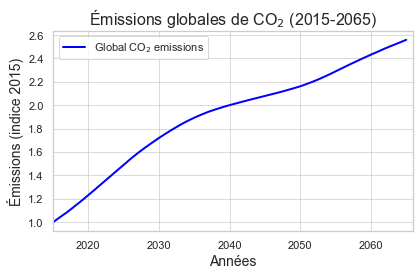
\includegraphics[width=0.8\textwidth]{images_IMACLIM/co2_baseline.png}
    \caption{Évolution des émissions de CO$_2$ dans le scénario baseline 139.}
    \label{fig:co2_baseline}
\end{figure}

La courbe des émissions globales de $CO_2$ sur la période 2015-2065 montre une tendance générale à la hausse, typique d'une \textit{baseline} où les politiques de réduction des émissions sont absentes. Cette trajectoire est influencée par les paramètres de notre \textit{baseline}, notamment la croissance rapide de la productivité et la forte disponibilité des combustibles fossiles, qui surpassent probablement les effets limités d’une faible amélioration de l’efficacité énergétique.

La représentation du taux de croissance annuel des émissions globales de CO$_2$ d'une part, et leur taux de croissance moyen de l'autre (\textit{cf.} fig. \ref{fig:croissance_co2_baseline}) permet de mieux appréhender les dynamiques sous-jacentes des émissions. 

\begin{figure}[H]
    \centering
    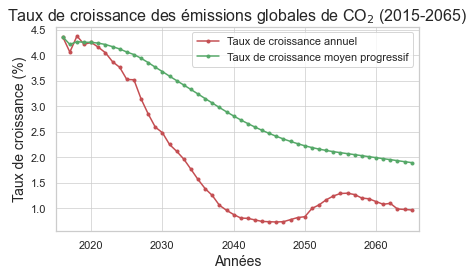
\includegraphics[width=0.8\textwidth]{images_IMACLIM/croissance_co2_baseline.png}
    \caption{Le taux de croissance annuel capture les fluctuations interannuelles des émissions de CO$_2$ : il mesure les dynamiques de court-terme et peut ainsi refléter les effets immédiats d'ajustement, de chocs exogènes (crises économiques, politiques climatiques) ou de changement technologique sur les émissions.
    Le taux de croissance moyen est calculé de façon cumulative, permettant de révéler la tendance structurelle, à long-terme, de la croissance des émissions.}
    \label{fig:croissance_co2_baseline}
\end{figure}

Le taux de croissance annuel nous permet de remarquer qu'après une période de 5 ans (2015 - 2020) de croissance stable et élevée des émissions, elle diminue drastiquement jusqu'en 2040 : on peut d'ores et déjà soulever l'hypothèse d'un effet cumulé de l'efficacité énergétique et des comportements de consommation frugaux ; un pic pétrolier peut aussi être à l'œuvre. Un sursaut du taux de croissance survient entre 2045 et 2055 : il peut être lié à un retour de la rentabilité des énergies fossiles, ou bien à une croissance économique non-décarbonée dominant les efforts d'économie d'énergie. 

Entre 2015 et 2065, le taux de croissance moyen est divisé par deux. Toutefois, à 2\% en 2065, il reste élevé et ne permet certainement pas de contenir le réchauffement climatique dans les limites fixées par l'accord de Paris. Pour s'en convaincre, on déduit l'augmentation de la température globale à partir de la réponse climatique transitoire aux émissions cumulées de CO$_2$ ($TCRE$)\footnote{Matthews, H., Gillett, N., Stott, P. et al. The proportionality of global warming to cumulative carbon emissions. Nature 459, 829–832 (2009). \url{https://doi.org/10.1038/nature08047}.}.
\begin{equation}
    \Delta T = TCRE \times \text{Emissions cumulées}
\end{equation}

Les émissions cumulées sont exprimées en gigatonnes de carbone (GtC), qu'on peut convertir en GtCO$_2$ en les multipliant par $\frac{44}{12}$ (rapport des masses molaires). D'après le sixième rapport du GIEC\footnote{IPCC, 2021: Summary for Policymakers. In: Climate Change 2021: The Physical Science Basis. Contribution of Working Group I to the Sixth Assessment Report of the Intergovernmental Panel on Climate Change [Masson-Delmotte, V., P. Zhai, A. Pirani, S.L. Connors, C. Péan, S. Berger, N. Caud, Y. Chen, L. Goldfarb, M.I. Gomis, M. Huang, K. Leitzell, E. Lonnoy, J.B.R. Matthews, T.K. Maycock, T. Waterfield, O. Yelekçi, R. Yu, and B. Zhou (eds.)]. In Press.}, $TCRE = 1.65 ~ [1.0 ~;~ 2.3]~ \tccentigrade/(10^{18}gC)$.

\begin{equation}
    \Delta T[\tccentigrade] = \frac{12}{44} \times 10^{-3}\times TCRE[\tccentigrade/TtC] \times \text{Emissions cumulées}[GtCO_2] 
\end{equation}

En sachant qu'en 2015, les émissions mondiales sont montées à 36.32 $GtCO_2$\footnote{The Global Carbon Budget 2023 (Friedlingstein et al., 2023b, ESSD), \url{https://explore.globalcarbonbudgetdata.org/timeseries.html}}, on en déduit la hausse de température présentée figure \ref{fig:temperature_baseline}. Or, sur la période 2006–2015, le réchauffement climatique était estimé à $0.87 \pm 0.12 ~ \tccentigrade$ par rapport à l'ère pré-industrielle\footnote{Allen, M.R., O.P. Dube, W. Solecki, F. Aragón-Durand, W. Cramer, S. Humphreys, M. Kainuma, J. Kala, N. Mahowald, Y. Mulugetta, R. Perez, M. Wairiu, and K. Zickfeld, 2018: Framing and Context. In: Global Warming of 1.5°C. An IPCC Special Report on the impacts of global warming of 1.5°C above pre-industrial levels and related global greenhouse gas emission pathways, in the context of strengthening the global response to the threat of climate change, sustainable development, and efforts to eradicate poverty [Masson-Delmotte, V., P. Zhai, H.-O. Pörtner, D. Roberts, J. Skea, P.R. Shukla, A. Pirani, W. Moufouma-Okia, C. Péan, R. Pidcock, S. Connors, J.B.R. Matthews, Y. Chen, X. Zhou, M.I. Gomis, E. Lonnoy, T. Maycock, M. Tignor, and T. Waterfield (eds.)]. Cambridge University Press, Cambridge, UK and New York, NY, USA, pp. 49-92, \url{doi:10.1017/9781009157940.003}.}. Ainsi, en 2060, la température mondiale pourrait atteindre $+ 1.55 \text{ à } +2.9 ~ \tccentigrade$ par rapport à l'ère pré-industrielle, nuisant de fait à l'objectif de maintenir si possible le réchauffement à 1.5 $\tccentigrade$.

\begin{figure}[H]
    \centering
    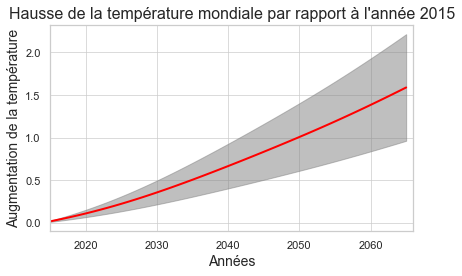
\includegraphics[width=0.8\textwidth]{images_IMACLIM/temperature_baseline.png}
    \caption{Possible augmentation de la température mondiale due aux émissions de CO$_2$ dans le scénario \textit{baseline} 139.}
    \label{fig:temperature_baseline}
\end{figure}


\subsection{Décomposition de Kaya des émissions}
Les émissions totales peuvent se décomposer selon le produit suivant :
\begin{align*}
    (\text{Population}) \times (\text{PIB/habitant}) \times (\text{Intensité énergétique du PIB}) \times (\text{Intensité carbone de l’énergie})
\end{align*} 
\ans{Tracer l’évolution dans le temps de ces quatre facteurs de la décomposition de Kaya sur un même graphique. Commentez.}

\begin{figure}[H]
    \centering
    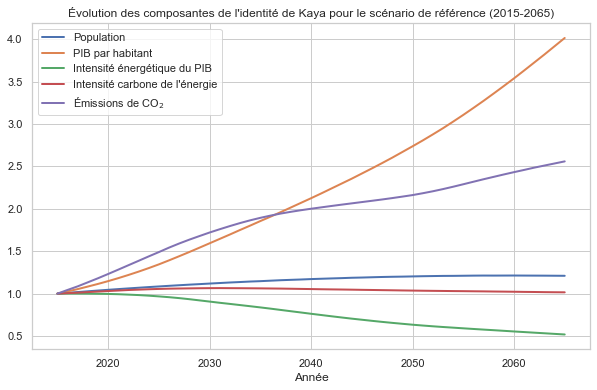
\includegraphics[width=\textwidth]{images_IMACLIM/kaya_baseline.png}
    \caption{Décomposition de Kaya.}
    \label{fig:kaya_baseline}
\end{figure}

À notre décomposition de Kaya (\textit{cf.} fig. \ref{fig:kaya_baseline}) nous ajoutons la contribution de chaque facteur à la variation des émissions de CO$_2$ sur trois périodes de références, identifiées à partir de la figure \ref{fig:croissance_co2_baseline}. Les résultats associés sont résumés dans le tableau \ref{tab:contributions_emissions}.

Remarquons en premier lieu la quasi-constance de l’intensité carbone, qui pour rappel mesure la proportion de $CO_2$ par unité d'énergie, c'est-à-dire à quel point les sources d'énergie sont carbonées. Dans ce scénario sans politique climatique, la dépendance aux combustibles fossiles prédomine, freinant l’adoption des technologies bas carbone. Malgré leur disponibilité, les rigidités structurelles (du travail et du gain d'efficacité énergétique) empêchent une transition vers des sources moins carbonées, alors que les énergies fossiles ne viennent pas à manquer. Le mix énergétique en 2065 est donc peu ou prou le même qu'en 2015 d'un point de vue agrégé. 

La variation de la population correspond à celle du scénario SSP5, une croissance démographique modérée, mais qui compte tout de même pour 1/7$^{\text{ème}}$ de la variation des émissions de CO$_2$ entre 2020 et 2045, venant soutenir un accroissement de la demande énergétique. 

La croissance rapide du PIB par habitant est le facteur dominant expliquant l'augmentation des émissions, d'autant qu'elle est élevée dans tous les pays (les pays convergeant rapidement vers le leader, dont la productivité est élevée). Cette croissance est cohérente avec un modèle économique dépendant d'énergies fossiles largement disponible. 

L'intensité énergétique est le facteur principal s'opposant à la croissance des émissions de CO$_2$, particulièrement sur la période 2020-2045. Elle est le reflet d'une production plus efficiente, soutenue notamment par le secteur du fret dont le besoin diminue avec l'augmentation de la productivité du travail et l'efficacité énergétique dans un scénario de frugalité. \\

Ainsi, l’interaction entre ces facteurs dans le cadre de la \textit{baseline} met en évidence un futur où la croissance économique et l'accroissement démographique exacerbent les émissions de $CO_2$, l'absence de réduction de l'intensité carbone ne permettant d'atteindre les objectifs de réduction d’émissions. 

\begin{table}[H]
\centering
\begin{tabularx}{\textwidth}{X*{5}{>{\centering\arraybackslash}X}}
    \toprule
      Période &  Contribution Population (\%) &  Contribution PIB par habitant (\%) &  Contribution Intensité énergétique (\%) &  Contribution Intensité carbone (\%) &  Variation cumulée des émissions de CO$_2$ (\%) \\
    \midrule
    2015-2020 &                         4.76 &                              15.57 &                                   -0.38 &                                3.23 &                                          23.18 \\
    2020-2045 &                        10.00 &                              79.85 &                                  -22.05 &                                0.99 &                                          68.79 \\
    2045-2065 &                         1.00 &                              38.16 &                                  -14.48 &                               -1.61 &                                          23.07 \\
    \bottomrule
\end{tabularx}
\caption{Contributions des différents facteurs à la variation des émissions de CO$_2$ sur différentes périodes. La somme des contributions est égale à la variation totale des émissions de CO$_2$.}
\label{tab:contributions_emissions}
\end{table}

\subsection{Analyse des "phases" d'évolution des intensités énergétiques et carbone}

\ans{Tracez l’évolution de l’intensité carbone de l’énergie en fonction de l’évolution de l’intensité énergétique du PIB mondial. Pouvez-vous identifier plusieurs phases dans l’évolution de ces deux facteurs ? Pouvez-vous proposer une hypothèse de mécanismes expliquant ces évolutions ? Que feriez-vous pour vérifier votre hypothèse ?}

Nous représentons l’évolution de l’intensité carbone de l’énergie et fonction de l’évolution de l’intensité énergétique du PIB figure \ref{fig:intensites}. La courbe débute au point $(1,1)$, correspondant à l'année 2015 : le graphique se lit ainsi de droite à gauche. Chaque point correspond à une année ; on comprend donc que plus une zone est dense en point, moins l'évolution est rapide.

\begin{figure}[H]
    \centering
    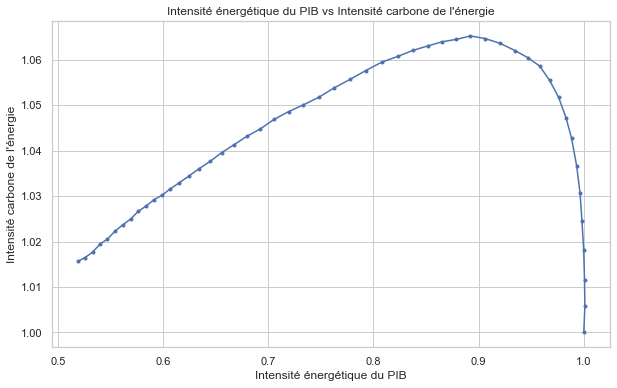
\includegraphics[width=\textwidth]{images_IMACLIM/intensites_baseline.png}
    \caption{Relation entre intensité carbone et intensité énergétique du PIB.}
    \label{fig:intensites}
\end{figure}

\begin{figure}[H]
    \centering
    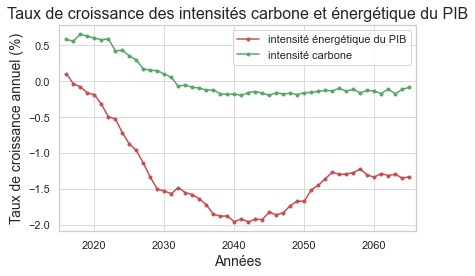
\includegraphics[width=0.8\textwidth]{images_IMACLIM/croissance_intensites.png}
    \caption{Évolution du taux de croissance annuel de l'intensité carbone et de l'intensité énergétique du PIB.}
    \label{fig:croissance_intensites}
\end{figure}

Afin de déterminer les différentes phases d'évolution de ces deux facteurs, nous nous intéressons à leur taux de croissance annuel, représenté figure \ref{fig:croissance_intensites}. On identifie alors trois phases distinctes :
\begin{enumerate}
    \item 2015 - 2030 : le taux de croissance de l'intensité carbone diminue jusqu'à 0, \textit{i.e.} elle atteint son maximum en 2030. Le taux de croissance de l'intensité énergétique, négatif, diminue drastiquement, témoignant d'une accélération de la diminution de la consommation d'énergie par unité de PIB. 
    \item 2030 - 2055 : l'intensité carbone diminue très faiblement à taux fixe, tandis que l'intensité énergétique continue de décroître rapidement, atteignant sa vitesse maximale en 2040, avant de revenir à une décroissance plus modérée.
    \item 2055 - 2065 : les deux intensités diminuent à taux constants.
\end{enumerate}

Nous représentons ces phases à travers trois régressions linéaires, figure \ref{fig:regression_intensite}.

\begin{figure}[H]
    \centering
    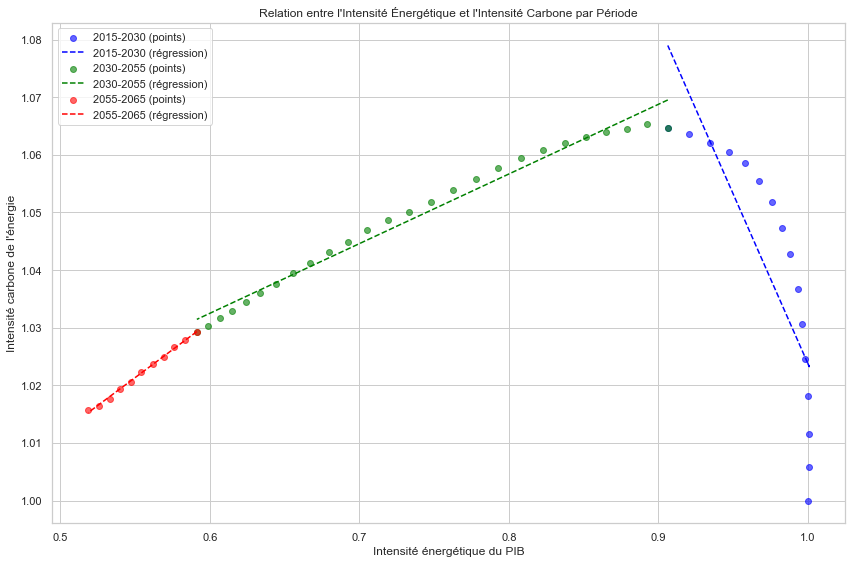
\includegraphics[width=\textwidth]{images_IMACLIM/regression_intensite.png}
    \caption{Relation entre intensité carbone et intensité énergétique du PIB, exacerbée par des régressions linéaires.}
    \label{fig:regression_intensite}
\end{figure}

\begin{enumerate}
    \item Phase initiale (2015 - 2030) : sur cette période, l'intensité énergétique diminue de 10\% alors que l'intensité carbone augmente de 6\%. On peut supposer là une potentielle différentiation entre les pays du Nord et du Sud. Les premiers, par la croissance de la productivité, obtiennent des gains d'efficacité énergétique, couplés à des comportements sobres. Les seconds, dont la vitesse de rattrapage est élevée et donc la croissance très forte, passent par une phase de développement intensive en énergies fossiles (comme les pays du Nord aux XIX-XX$^{\text{èmes}}$ siècles).
    \item Phase de transition (2030 - 2055) : l'intensité énergétique diminue de 33\% alors que l'intensité carbone ne baisse que de 3\%. Cette chute drastique peut traduire le passage généralisé à une économie de service / dématérialisée, ou bien simplement moins énergivore : ce régime transitoire enclenche une convergence de l'économie mondiale vers une intensité énergétique faible par une optimisation de la consommation d'énergie. Le comportement de l'intensité carbone traduit néanmoins une dépendance continue aux énergies fossiles, qui malgré la disponibilité des technologies bas-carbone, restent compétitives.
    \item Phase de stabilisation (2055 - 2065) : les deux intensités diminuent à taux constant, respectivement de 13\% et 1.5\%. Alors que la croissance continue modifie les structures économiques, notamment les technologies de production, l'intensité carbone reste stable, témoignant d'un rejet des technologies bas-carbone (à cause de leur manque de rentabilité ou bien de freins structurels).
\end{enumerate}

Pour vérifier les hypothèses soulevées sur la différentiation entre pays développés et émergents et sur des optimisations technologiques voire un changement de la structure de l'économie des biens vers les services, il serait intéressant d'observer les données déségragées par pays d'une part, par secteur de production de l'autre, puis éventuellement les interactions entre ces désagrégations : nous pourrions alors observer l'interaction d'effets de composition sectorielle et d'effets de composition régionale. 


\vspace{0.3cm}
\section{\Large{Analyse d’un scénario d’atténuation}}
\vspace{0.3cm}
\ans{Vous allez maintenant analyser le scénario d’atténuation correspondant à la baseline que vous avez choisie, son numéro de scénario est celui de la baseline + 216 (car il y a 216 scénarios de baseline dans l’ensemble de scénarios).}

Le scénario d'atténuation correspondant à la \textit{baseline} 139 est le scénario 355 : il garantit une trajectoire des émissions telle que le seuil des 550 ppm de CO$_2$ dans l'atmosphère ne soit pas dépassé, correspondant au dépassement des 2 $\tccentigrade$ de réchauffement par rapport à l'ère préindustrielle. Les valeurs des paramètres sont les mêmes que celles de la \textit{baseline}. Dans le cadre d'une politique d'atténuation (qui peut passer par un prix du carbone, une taxe, du \textit{cap-and-trade}, des normes ou des subventions)\footnote{\url{https://www.iamcdocumentation.eu/index.php/Reference_card_-_IMACLIM-NLU}}, on s'attend ainsi à ce que :
\begin{itemize}
    \item les énergies fossiles soient économiquement pénalisées, poussant à l'adoption d'énergies bas-carbone malgré la disponibilité élevée des premières et le coût initial des secondes (une contrainte qui peut être levée par des politiques climatiques).
    \item la croissance soutenue de l'économie mondiale soit décarbonée, par une transition plus rapide vers des sources d'énergie moins carbonées, couplée à des comportements frugaux.
    \item malgré la faible vitesse de gain d'efficacité énergétique, une politique publique visant à limiter les émissions peut stimuler cette efficacité auprès des agents (lorsque leur consommation carbonée est pénalisée par exemple).
    \item les rigidités sur le marché du travail soient des sources potentielles de chômage si ne sont pas mises en place des politiques de reconversion des travailleurs vers des secteurs plus verts.
\end{itemize} 

Ainsi, voilà les effets majeurs que l'on pressent : 

\begin{enumerate}
    \item \textbf{Décarbonation forcée des secteurs économiques} : des politiques de \textit{pricing} peuvent servir de levier pour forcer la réduction de l’intensité carbone des industries, même avec une disponibilité élevée de combustibles fossiles.
    \item \textbf{Stimulation de l’adoption des technologies bas carbone} : les technologies propres deviennent plus attractives économiquement et voient leur adoption s’accélérer à l'aide d’incitations financières.
    \item \textbf{Influence sur le comportement énergétique} : l'efficacité des comportement sobres est renforcé par la décarbonation des secteurs sur lesquels ils reposent (transports et véhicules électriques, efficacité énergétique des bâtiments, biens industriels moins intensifs en énergie carbonée et fret plus "vert").
    \item \textbf{Convergence de croissance plus durable} : Le rattrapage rapide de la productivité dans les régions émergentes se déroule dans un contexte où les choix technologiques et énergétiques tendent vers des options bas carbone, renforçant un développement économique plus durable.
\end{enumerate}

\subsection{Décomposition de Kaya des émissions}

\ans{Tracer l’évolution dans le temps des quatre facteurs de la décomposition de Kaya des émissions dans ce scénario d’atténuation sur un même graphique. Commentez, et comparez avec la baseline.}

Notre décomposition peut être trouvée figure \ref{fig:kaya_attenuation} : elle présente des divergences significatives par rapport à la \textit{baseline}. On approndit son analyse à l'aide de la figure \ref{fig:emissions_taux_attenuation}, qui permet un zoom sur l'évolution des émissions et de leur taux de croissance annuel.
Notons en premier lieu que la population étant exogène, elle ne varie pas entre les deux scénarios.

On distingue une première période entre 2015 et 2027, où l'on assiste à une légère hausse des émissions de $CO_2$, jusqu'à un pic en 2020, avant de retrouver en 2027 le niveau d'émissions de 2015. Entre 2027 et 2045 s'ensuit une accélération de la baisse des émissions mondiales, le taux de croissance annuel passant de -0.5\% à -2.8\%. Après 2045, la baisse des émissions se stabilise autour d'une décroissance annuelle de 2.5\%, jusqu'à atteindre moins de la moitié des émissions de 2015 en 2065. Le lag de 5 ans de croissance des émissions peut correspondre au temps de déploiement d'une politique climatique, couplée au temps de déploiement des technologies bas-carbone, dont la phase de développement est supposée non-nulle par le modèle (2 ans pour les renouvelables, 6 ans pour les véhicules électriques, 13 ans pour le CCS et 15 pour le nucléaire nouvelle génération).

\begin{figure}[H]
    \centering
    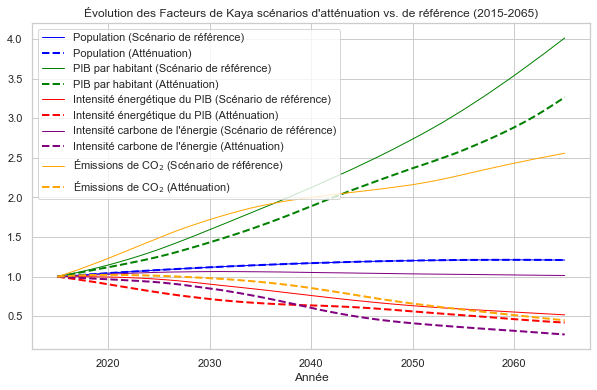
\includegraphics[width=\textwidth]{images_IMACLIM/kaya_attenuation.png}
    \caption{Décomposition de Kaya dans le scénario baseline (139) et le scénario d'atténuation (355).}
    \label{fig:kaya_attenuation}
\end{figure}

\begin{figure}[H]
    \centering
    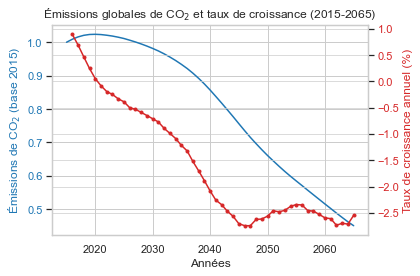
\includegraphics[width=0.8\textwidth]{images_IMACLIM/emissions_taux_attenuation.png}
    \caption{Évolution des émissions et de leur taux de croissance annuel dans un scénario d'atténuation.}
    \label{fig:emissions_taux_attenuation}
\end{figure} 

La croissance du PIB par habitant est constamment légèrement inférieure dans le scénario d'atténuation. On peut supposer que l'introduction d'un prix du carbone augmente les coûts de production, freinant la productivité dans les industries à haute intensité carbone (notamment dans les pays du Sud), et que le progrès technique ne compense pas ces pertes. Il nous faut aussi ajouter que les marchés sont rigides : la réallocation des travailleurs des \textit{sunset industries} vers les autres secteurs de production peut entraîner des frictions, du chômage, etc. L'effet de la mitigation réduirait ainsi le PIB par habitant une fois les politiques climatiques mises en place. 

Par rapport à la \textit{baseline}, la diminution de l’intensité énergétique se fait plus rapidement, jusqu'à arriver à un niveau similaire (légèrement inférieur) en 2065. Des politiques augmentant le coût du carbone et favorisant les technologies bas carbone motiveraient les entreprises à investir dans des processus de production moins énergivores. Cependant, le gain d'efficacité énergétique restant un processus progressif, limité par les contraintes d’investissement et la lenteur de diffusion des technologies, une convergence entre les courbes advient sur le long-terme et suggère que, malgré les incitations, le potentiel d’efficacité énergétique ne peut dépacer un certain plateau (défini par la valeur de notre paramètre).

La variation la plus marquée entre \textit{baseline} et scénario d'atténuation est celle de l'intensité carbone. Plutôt constante dans le premier cas, elle diminue de manière signigicative dans le second, notamment entre 2027 et 2045 : elle semble être le moteur principal de la baisse des émissions de CO$_2$ dans ce scénario. Le comportement de l'intensité carbone est celui qui peut être expliqué le plus simplement, les politiques publiques de mitigation visant explicitement à réduire la part des énergies fossiles dans le mix énergétique mondial (elles peuvent moins facilement diriger l'intensité énergétique du PIB, où des effets rebonds indirect pourraient  par exemple advenir).

On suppose ainsi que le déploiement de politiques climatiques entraîne du progrès technique (par R\&D) dans les technologies bas-carbone, de la profitabilité des énergies renouvelables, et par conséquent une restructuration de l'économie qui se tourne vers des secteurs de production plus durables. L’intensité carbone et l’intensité énergétique du PIB sont alors réduites.


\subsection{Analyse de la variation de PIB entre le scénario d’atténuation et la baseline correspondante}

\ans{Calculez la trajectoire temporelle de variation de PIB mondial entre le scénario d’atténuation et la baseline correspondante. Tracez-la. Commentez. Convertir en perte de croissance annuelle moyenne à l’horizon 2030, 2050, 2065. Commentez.}

La figure \ref{fig:variation_PIB} permet de visualiser simultanément la trajectoire temporelle de variation du PIB mondial entre le scénario d'atténuation et la \textit{baseline} correspondante, et la perte de croissance annuelle moyenne à divers horizon. 

On retrouve peu ou prou les mêmes périodes d'analyse que celles identifiées pour analyser les émissions de GES dans un cas de mitigation.
\begin{enumerate}
    \item 2015 - 2027 : on assiste au premier décrochage du PIB issu du scénario d'atténuation par rapport à la \textit{baseline}. La différenciation ne fait que s'accélerer sur cette période, jusqu'à présente une différence de taux de croissance moyen de 75\% en 2027~! Il est possible que l'introduction de politiques climatiques et leur temps de déploiment impliquent de lourds impacts sur la croissance économique à travers des coûts supplémentaires sur les secteurs polluants (dans un cadre où les énergies fossiles sont pourtant abondantes), obligeant les entreprises à investir dans des technologies plus propres aux dépens d'une croissance plus facile car soutenue par les fossiles, à restructurer leur production, et à ajuster leur main-d'œuvre. 
    \item 2027 - 2045 : les deux scénarios maintiennent une variation de PIB relativement constante, le scénario d'atténuation se maintenant à un PIB aux alentours de 11\% inférieur à la \textit{baseline}. Les technologies bas-carbone déployées et les gains d'efficacité énergétique majoritairement réalisés (donc le progrès technique) permet de maintenir une trajectoire de croissance relativement similaire à la \textit{baseline}. Néanmoins, le non-recours aux énergies fossiles (pourtant abondantes et ainsi employées dans le scénario sans politiques climatiques) ne permet pas d'atteindre le niveau de PIB de la \textit{baseline}. La perte de croissance annuelle moyenne à horizon 2045/2050 est ainsi de 42\% : par rapport à l'horizon 2030, on constate un rattrapage du taux de croissance du PIB sous le scénario d'atténuation (il était auparavant à 73\%), mais qui traduit toutefois un écart de croissance marqué par rapport à la \textit{baseline}.
    \item 2045 - 2065 : on assite au second décrochage du PIB 'atténuation', qui passe de -11\% à -18.5\% en 2065. Il est possible que l'on assiste au contrecoup des politiques climatiques. Sans elles, les pays du Nord comme les pays du Sud bâtissent encore leur forte croissance sur des énergies fossiles toujours disponibles, tendant vers une convergence mondiale de la croissance (\textit{i.e.} les pays ont tous atteint le stade de société de consommation, et l'absence de fonction de dommages climatiques dans le modèle ne pénalise pas une croissance soutenue et très carbonée). Au contraire, leur application dans un monde économique peu flexible peut entraîner à terme des pertes de croissance importantes, surtout si la majorité des bénéfices de cette transition énergétiques ont déjà été récoltés (les effets des gain d'efficacité et du progrès technique se manifestent principalement sur la période 2027-2045, avant d'atteindre un plateau par la suite). On note toutefois que sur cette période, la perte de croissance annuelle moyenne est comprise entre 40\% et 50\%. Cet intervalle de valeur, proche de celle de la période précédente, traduit une certaine stabilité de l'écart du taux de croissance moyen entre les deux scénarios, et signifie probablement que le décrochage principal du PIB sous scénario d'atténuation a eu lieu avant 2027.
\end{enumerate}

\begin{figure}[H]
    \centering
    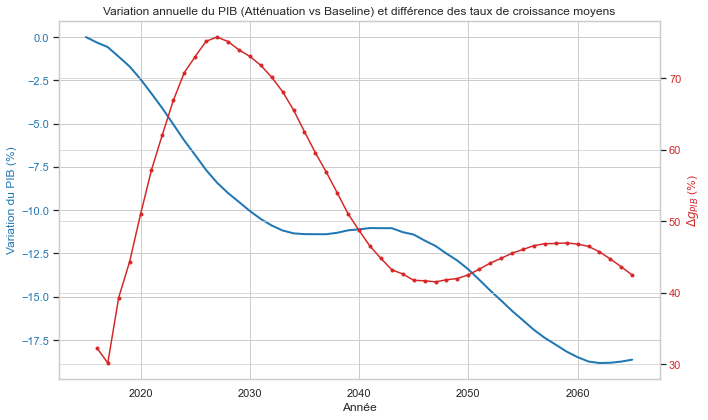
\includegraphics[width=\textwidth]{images_IMACLIM/variation_PIB.png}
    \caption{Gauche : Écart de PIB entre le scénario d'atténuation et la \textit{baseline}. Droite : Écart des taux de croissance moyens du PIB sans et avec politique de mitigation (\%).}
    \label{fig:variation_PIB}
\end{figure}

\vspace{0.3cm}
\section{{Analyse d’une base de données (d’un ensemble) de scénarios}}
\vspace{0.3cm}

\subsection{Scénarios de baseline dans l’espace « émissions cumulées vs croissance annuelle moyenne »}

\ans{Calculez les émissions cumulées sur la période 2015-2065 dans les scénarios, et la croissance annuelle moyenne sur 2015-2065 dans les scénarios. Placez les scénarios de baseline dans l’espace « émissions cumulées vs croissance annuelle moyenne », \textit{i.e.} chaque scénario est un point avec pour l’axe des abscisses la croissance annuelle moyenne et pour l’axe des ordonnées les émissions cumulées.}

La figure \ref{fig:baselines_scenarios} présente l'ensemble des scénarios de \textit{baseline} selon leurs émissions cumulées entre 2015 et 2065 et leur taux de croissance annuelle moyen. On remarque une forte dispersion entre les \textit{baselines} possibles ; notamment, une grande majorité du spectre \{[2800,~4000] GtCO$_2$ ; [1.75,~3]\%\} est couvert. Notons que pour rester en-dessous de 2 $\tccentigrade$ de réchauffement avec une probabilité de 66\%, il faudrait que les émissions cumulées entre 2015 et 2100 ne dépassent pas 1200 GtCO$_2$\footnote{Friedlingstein, P., Andrew, R., Rogelj, J. et al. Persistent growth of CO2 emissions and implications for reaching climate targets. Nature Geosci 7, 709–715 (2014). \url{https://doi.org/10.1038/ngeo2248}}. Aucun scénario de \textit{baseline} ne permet cela.

\begin{figure}[H]
    \centering
    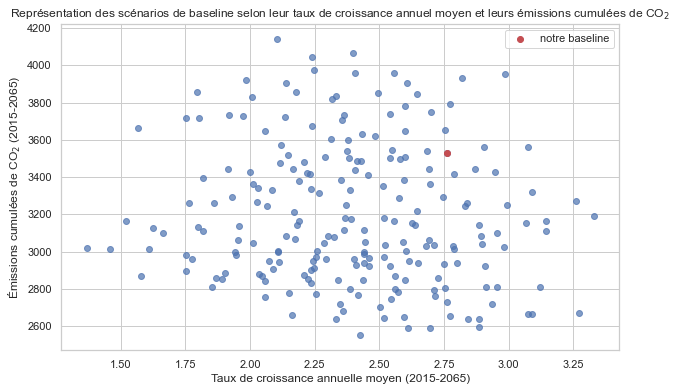
\includegraphics[width=0.9\textwidth]{images_IMACLIM/baselines_scenarios.png}
    \caption{Ensemble des scénarios de \textit{baseline} représentés par leurs émissions cumulées et leur croissance annuelle moyenne.}
    \label{fig:baselines_scenarios}
\end{figure}


\subsection{Histogramme des croissances annuelles moyennes}
\ans{Tracez sur un même histogramme (fonction \texttt{plt.hist}) les croissances annuelles \\
moyennes dans les scénarios de baseline et d’atténuation. Commentez.}

\begin{figure}[H]
    \centering
    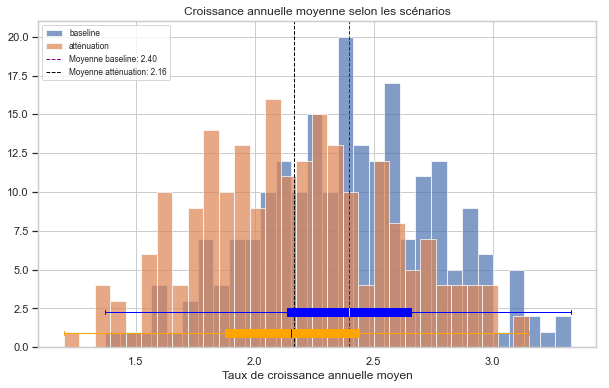
\includegraphics[width=0.9\textwidth]{images_IMACLIM/histo_growth.png}
    \caption{Représentation en histogrammes et en \textit{boxplots} du taux de croissance annuelle moyen selon le type de scénario.}
    \label{histo_growth}
\end{figure}

À partir de la figure \ref{histo_growth}, nous remarquons que : 
\begin{itemize}
    \item La distribution des taux de croissance annuelle moyens des scénarios d'atténuation est décalée sur la gauche par rapport à celle de la \textit{baseline}, quoique les histogrammes se chevauchent tout de même. Cela semble traduire une tendance générale à une croissance plus faible dans les scénarios d'atténuation, affectée par les politiques climatiques. Soulignons néanmoins encore une fois que le modèle IMACLIM-R ne prend pas en compte les bénéfices de la mitigation sur la croissance économiques, qu'ils soient directs (moins de dégradation sur le capital par les évènements climatiques extrêmes) ou indirects (effets sur la santé, etc.)
    \item Chaque distribution voit sa moyenne et sa médiane (quasi-)confondues, et l'écart interquartile est similaire entre les distributions : les scénarios ont donc été construits de manière relativement symétrique.
    \item Le taux de croissance annuel moyen le plus faible reste supérieur à 1\% dans les deux cas : aucun scénario de décroissance économique n'advient.
\end{itemize}


\subsection{Anova}
\ans{Choisissez une variable de sortie, soit les émissions soit la croissance, dans un sous-ensemble des scénarios, soit les baselines soit les scénarios d’atténuation. Construisez l’analyse de la variance, anova, de cette variable dans ce sous-ensemble des scénarios afin d’analyser les contributions des différents groupes de paramètres à la variance du résultat. Vous pourrez demander un exemple de code qui construit des anova. Commentez.}

\begin{figure}[H]
        \centering
        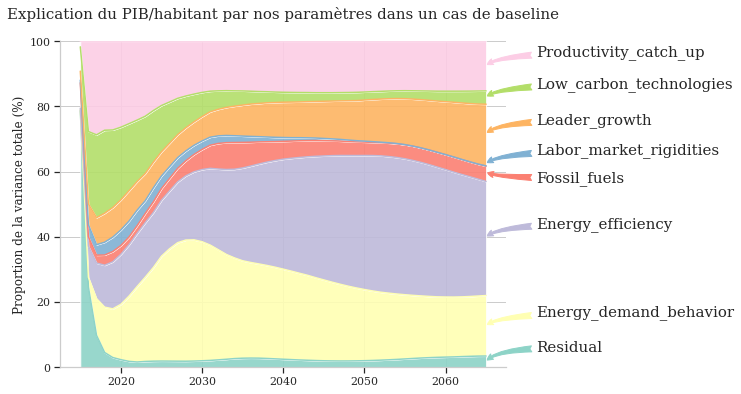
\includegraphics[width=\textwidth]{images_IMACLIM/anova_baseline.png}
        \caption{ANOVA sur le PIB/habitant - \\
        baselines.}
        \label{fig:anova_baseline}
\end{figure}

\begin{figure}[H]
        \centering
        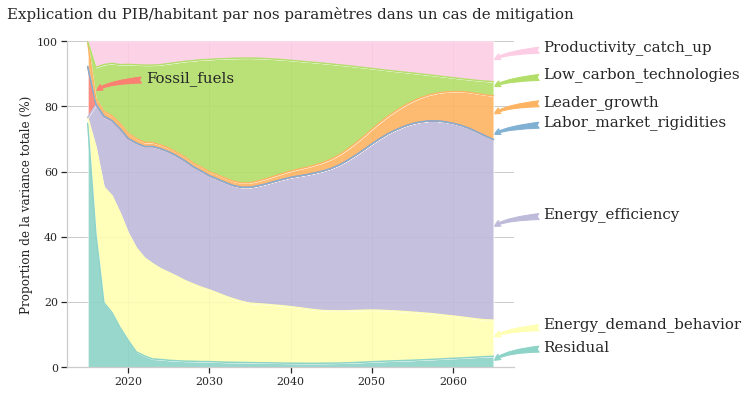
\includegraphics[width=\textwidth]{images_IMACLIM/anova_mitigation.png}
        \caption{ANOVA sur le PIB/habitant - \\
        scénarios d'atténuation.}
        \label{fig:anova_mitigation}
\end{figure}

Nous choisissons de performer une décomposition de la variance par ANOVA sur le PIB/habitant, pour les scénarios de \textit{baseline} d'une part (voir fig. \ref{fig:anova_baseline}) et les scénarios d'atténuation d'autre part (fig. \ref{fig:anova_mitigation}), afin de clairement identifier les variations des contributions des différents groupes de paramètres à la variance du résultat. Les effets d'interactions ont été exclus car leur pouvoir explicatif était infime. Soulignons d'ores et déjà le très faible pouvoir explicatif des rigidités de marché (pourtant élevées dans notre configuration), et que nous exclurons donc de notre analyse.

On retrouve alors des phases d'évolution identifiées précedemment, et les graphiques viennent appuyer certaines hypothèses ou au contraire en infirmer d'autres. 

\begin{enumerate}
    \item 2015 - 2020 : 
    \begin{itemize}
        \item Dans le scénario sans politiques climatiques, l'accroissement de productivité de l'ensemble des pays, notamment des pays émergents est un des principaux facteurs influançant la croissance économique. Le PIB/habitant est aussi fortement sensible aux hypothèses sur le développement des technologies bas-carbone, de tel sorte à ce que le progrès technique en technologies bas-carbone et la croissance de la productivité expliquent 60\% de la variance du PIB par habitant. De manière contre-intuitive, le recours aux énergies fossiles est un paramètre peu explicatif de la croissance économique. Considérant que le choix de développer ou non des technologies bas-carbone peut avoir un impact sur la productivité\footnote{Henriet, F., Maggiar, N. and Schubert, K. (2014), A Stylized Applied Energy-Economy Model for France, The Energy Journal, 35(4).}, on suppose que les choix de productions déterminent majoritairement les trajectoires de croissance sur cette courte période.
        \item Lorsqu'une contrainte de 550 ppm est instaurée, la répartition des moteurs clés de la croissance change drastiquement. L'arrêt des énergies fossiles advient dès 2018 et le rattrapage de productivité ne peut se construire sur les fossiles. Au contraire, les comportements de demande en énergie et l'efficacité énergétique expliquent 60\% de la variance du PIB : c'est donc les choix de sobriété et d'optimisation qui sous-tendent les chemins possibles de croissance.
    \end{itemize}
    Notons aussi la prégnance du résidu sur cette période, qui s'explique simplement par la phase de "calibration" du modèle. Les mécanismes de croissance endogène ne permettent pas une estimation robuste lors des premières itérations.
    \item 2020 - 2027 : 
    \begin{itemize}
        \item \textit{Baseline} : on assiste à une transfert entre les technologies bas-carbone, qui perdent drastiquement en importance, et les comportements frugaux des agents, qui viennent expliquer plus de 30\% de la variance du PIB : la demande influence la croissance. Les autres facteurs restent globalement constant, quoiqu'on assiste à une légère diminution de la part de la productivité. 
        \item Atténuation : dans ce scénario, le transfert se fait dans l'autre sens, et on voit la part de l'efficacité énergétique croître fortement. Supposant que le travail investi dans le développement des technologies bas-carbone fait perdre en croissance car il ne permet pas de gains de productivité du travail\footnote{\textit{ibid.}}, on peut soulever l'hypothèse de trajectoires de croissance dirigées par les paramètres régissant l'application des politiques climatiques et le déploiement des technologies bas-carbone (par exemple, les politiques de taxe carbone peuvent entraîner un choc négatif sur la demande d'énergie si le coût de l'énergie est élevé et/ou un choc positif sur l'innovation si des politiques de taxe carbone ont été mises en œuvre\footnote{Fried, Stephie. 2018. "Climate Policy and Innovation: A Quantitative Macroeconomic Analysis." American Economic Journal: Macroeconomics, 10 (1): 90–118. DOI: \url{10.1257/mac.20150289}}).
    \end{itemize}
    \item 2027 - 2045 :
    \begin{itemize}
        \item \textit{Baseline} : On assiste à un léger regain des énergies fossiles et de la croissance des USA dans la part de variance totale expliquée. Les énergies renouvelables ne sont pas impérativement nécessaires dans un monde sans politiques d'atténuation et où les énergies fossiles sont abondantes, or, il est probable que la productivité soit plus élevée lorsqu'elle est soutenue par des énergies fossiles : le niveau de consommation de ces dernières influence les trajectoires de croissance. Sur cette même période, les gains d'efficacité énergétiques expliquent jusqu'à 30\% de la variance du PIB/habitant. De forts gains énergétiques permettent de produire autant avec moins d'énergie, \textit{i.e.} de produire plus avec autant d'énergie. On en déduit finalement que les trajectoires de croissance sont déterminées par l'efficacité de la production. Le rôle de la demande énergétique reste importante.
        \item Scénario d'atténuation : Comme pour la \textit{baseline}, les comportements de consommation d'énergie voient leur pouvoir explicatif légèrement diminuer, passant à $\sim$ 20\% de la variance. La valeur du PIB/habitant dépend très majoritairement (70\% de la variance) des trajectoires d'amélioration des intensités énergétiques et carbone (gains d'efficacité énergétique et déploiement des énergies bas-carbone). On peut supposer qu'à la fin de cette période, les pays du Sud ont pu adopter les technologies bas-carbone dans la majorité des scénarios (d'où la diminution de pouvoir explicatif, $\sim$ 20\% en 2045 contre 50\% en 2027), et les trajectoires de gains d'efficacité énergétique (qui permettent de croître à quantité d'énergie donné) déterminent majoritairement le niveau de croissance (afin qu'elle soit compatible avec les limites d'émissions).
    \end{itemize}
    \item 2045 - 2065 :
    \begin{itemize}
        \item \textit{baseline} : La part de la productivité des USA et de l'efficacité énergétique croît dans l'explication de la variance, aux dépens de la demande en énergie des consommateurs. On poursuit globalement la tendance étudiée sur la période précédente.
        \item Scénario d'atténuation : similairement au cas sans politiques climatiques, la croissance de la productivité totale (celle des USA et celle des autres pays, qui converge vers le \textit{leader}) et l'efficacité énergétique dominent l'explication du PIB/habitant. Soulevons l'hypothèse que 30 ans après le début de la simulation, les progrès sur l'intensité carbone par le déploiement des technologies associées ont été menés sur l'ensemble des scénarios afin de contrôler la baisse des émissions. Les trajectoires de croissance sont alors fortement dépendantes des gains d'efficacité énergétique et des gains de productivité (notamment du travail).
    \end{itemize}
\end{enumerate}
\end{document}